
%<<setup-child, include = FALSE>>=

%library(knitr)
%options(digits = 16)

%library(RCurl)
%library(XML)
%library(tm)
%library(NMF)
%library(microbenchmark)
%library(ggplot2)
%library(wordcloud)
%set_parent("../style/preamble.Rnw")
%@


\newcommand{\xdownarrow}[1]{%
	{\left\downarrow\vbox to #1{}\right.\kern-\nulldelimiterspace}
}

\newcommand{\grey}[1]{\textcolor{grey}{#1}}
\newcommand{\red}[1]{\textcolor{red}{#1}}

\input{../../2021/style/preamble4tex}
% dependencies: amsmath, amssymb, dsfont
% math spaces
\ifdefined\N
\renewcommand{\N}{\mathds{N}} % N, naturals
\else \newcommand{\N}{\mathds{N}} \fi
\newcommand{\Z}{\mathds{Z}} % Z, integers
\newcommand{\Q}{\mathds{Q}} % Q, rationals
\newcommand{\R}{\mathds{R}} % R, reals
\ifdefined\C
\renewcommand{\C}{\mathds{C}} % C, complex
\else \newcommand{\C}{\mathds{C}} \fi
\newcommand{\continuous}{\mathcal{C}} % C, space of continuous functions
\newcommand{\M}{\mathcal{M}} % machine numbers
\newcommand{\epsm}{\epsilon_m} % maximum error

% counting / finite sets
\newcommand{\setzo}{\{0, 1\}} % set 0, 1
\newcommand{\setmp}{\{-1, +1\}} % set -1, 1
\newcommand{\unitint}{[0, 1]} % unit interval

% basic math stuff
\newcommand{\xt}{\tilde x} % x tilde
\newcommand{\argmin}{\mathop{\mathrm{arg\,min}}} % argmin
\newcommand{\argmax}{\mathop{\mathrm{arg\,max}}} % argmax
\newcommand{\argminlim}{\argmin\limits} % argmin with limits
\newcommand{\argmaxlim}{\argmax\limits} % argmax with limits
\newcommand{\sign}{\operatorname{sign}} % sign, signum
\newcommand{\I}{\mathbb{I}} % I, indicator
\newcommand{\order}{\mathcal{O}} % O, order
\newcommand{\bigO}{\mathcal{O}} % Big-O Landau
\newcommand{\littleo}{{o}} % Little-o Landau
\newcommand{\pd}[2]{\frac{\partial{#1}}{\partial #2}} % partial derivative
\newcommand{\floorlr}[1]{\left\lfloor #1 \right\rfloor} % floor
\newcommand{\ceillr}[1]{\left\lceil #1 \right\rceil} % ceiling
\newcommand{\indep}{\perp \!\!\! \perp} % independence symbol

% sums and products
\newcommand{\sumin}{\sum\limits_{i=1}^n} % summation from i=1 to n
\newcommand{\sumim}{\sum\limits_{i=1}^m} % summation from i=1 to m
\newcommand{\sumjn}{\sum\limits_{j=1}^n} % summation from j=1 to p
\newcommand{\sumjp}{\sum\limits_{j=1}^p} % summation from j=1 to p
\newcommand{\sumik}{\sum\limits_{i=1}^k} % summation from i=1 to k
\newcommand{\sumkg}{\sum\limits_{k=1}^g} % summation from k=1 to g
\newcommand{\sumjg}{\sum\limits_{j=1}^g} % summation from j=1 to g
\newcommand{\summM}{\sum\limits_{m=1}^M} % summation from m=1 to M
\newcommand{\meanin}{\frac{1}{n} \sum\limits_{i=1}^n} % mean from i=1 to n
\newcommand{\meanim}{\frac{1}{m} \sum\limits_{i=1}^m} % mean from i=1 to n
\newcommand{\meankg}{\frac{1}{g} \sum\limits_{k=1}^g} % mean from k=1 to g
\newcommand{\meanmM}{\frac{1}{M} \sum\limits_{m=1}^M} % mean from m=1 to M
\newcommand{\prodin}{\prod\limits_{i=1}^n} % product from i=1 to n
\newcommand{\prodkg}{\prod\limits_{k=1}^g} % product from k=1 to g
\newcommand{\prodjp}{\prod\limits_{j=1}^p} % product from j=1 to p

% linear algebra
\newcommand{\one}{\bm{1}} % 1, unitvector
\newcommand{\zero}{\mathbf{0}} % 0-vector
\newcommand{\id}{\bm{I}} % I, identity
\newcommand{\diag}{\operatorname{diag}} % diag, diagonal
\newcommand{\trace}{\operatorname{tr}} % tr, trace
\newcommand{\spn}{\operatorname{span}} % span
\newcommand{\scp}[2]{\left\langle #1, #2 \right\rangle} % <.,.>, scalarproduct
\newcommand{\mat}[1]{\begin{pmatrix} #1 \end{pmatrix}} % short pmatrix command
\newcommand{\Amat}{\mathbf{A}} % matrix A
\newcommand{\Deltab}{\mathbf{\Delta}} % error term for vectors

% basic probability + stats
\renewcommand{\P}{\mathds{P}} % P, probability
\newcommand{\E}{\mathds{E}} % E, expectation
\newcommand{\var}{\mathsf{Var}} % Var, variance
\newcommand{\cov}{\mathsf{Cov}} % Cov, covariance
\newcommand{\corr}{\mathsf{Corr}} % Corr, correlation
\newcommand{\normal}{\mathcal{N}} % N of the normal distribution
\newcommand{\iid}{\overset{i.i.d}{\sim}} % dist with i.i.d superscript
\newcommand{\distas}[1]{\overset{#1}{\sim}} % ... is distributed as ...


\begin{document}

\lecturechapter{7}{Topic Extraction}
\lecture{CIM1 Statistical Computation}



\begin{vbframe}{Application: Topic Extraction}

Often online articles refer to articles with similar content, e.g.

\begin{center}
	\textbf{\emph{\href{https://www.nytimes.com/2017/11/05/technology/machine-learning-artificial-intelligence-ai.html?rref=collection\%2Fsectioncollection\%2Ftechnology&action=click&contentCollection=technology&region=rank&module=package&version=highlights&contentPlacement=2&pgtype=sectionfront}{Building AI that Can Build AI}}} \\
	$\Big\downarrow$ \footnotesize{\enquote{related}}\\
	\normalsize \textbf{	\emph{\href{https://www.nytimes.com/2017/09/10/business/warehouse-robots-learning.html?action=click&contentCollection=Technology&module=RelatedCoverage&region=Marginalia&pgtype=article}{In the Future, Warehouse Robots Will Learn on Their Own}}} \\
	$\Big\downarrow$ \footnotesize \enquote{related}\\
	\normalsize\textbf{	\emph{\href{https://www.nytimes.com/2017/09/10/technology/amazon-robots-workers.html?action=click&contentCollection=Business\%20Day&module=RelatedCoverage&region=Marginalia&pgtype=article}{As Amazon Pushes Forward With Robots, Workers Find New Roles}}}
\end{center}

The first two articles should definitely have one topic in common, just like the last two articles. We want to extract these two topics using a NMF.

\framebreak

We set up the corresponding document-term matrix.

\lz

\footnotesize
\begin{verbatim}
##                doc1 doc2 doc3
## accelerate      1    0    0
## accelerating    1    0    0
## accurately      1    0    0
## across          1    1    2
## address         1    1    0
## adjust          1    0    0
\end{verbatim}

%<<echo = F>>=
%options(digits = 2)
%@

%<<echo = F>>=
%tdm = readRDS("rsrc/tdm")
%@

%<<echo=F>>=
%head(tdm)
%@

\framebreak

We \enquote{search} two topics linking the articles.
\vspace{0.2cm}

\footnotesize
\begin{verbbox}
set.seed(1)
res = nmf(tdm, 2, "Frobenius")
\end{verbbox}
\col

\lz
\begin{verbatim}
##                topic1   topic2
## accelerate     0.0016   3.8e-11
## accelerating   0.0016   3.8e-11
## accurately     0.0016   3.8e-11
## across         0.0023   4.1e-03
## address        0.0026   6.3e-05
## adjust         0.0016   3.8e-11
\end{verbatim}

%<<>>=
%set.seed(1)
%res = nmf(tdm, 2, "Frobenius")
%@

%<<echo = F>>=
%wordmatrix = as.data.frame(basis(res)) # topic-word-matrix

%wordmatrix$word = rownames(wordmatrix)
%colnames(wordmatrix) = c("topic1", "topic2", "word")

%head(wordmatrix)[1:2]
%@

\normalsize
\end{vbframe}

\begin{vbframe}{Topic Extraction: Topic 1}

For both topics, we print the $30$ words with the largest values in the columns of matrix $\mathbf{W}$. The size of the word in the wordcloud is determined by the value of $w_{ij}$ (placement of the word is completely random).\\

\begin{center}
	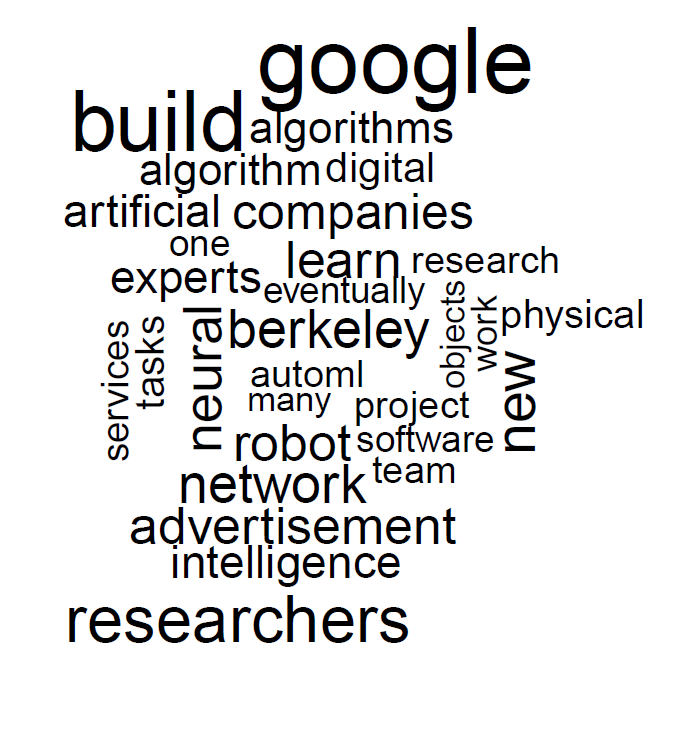
\includegraphics[width = 0.4\textwidth]{figure_man/wordcloud01.png}
\end{center}

%<<echo = F, out.width='70%', fig.align='center'>>=
%df = wordmatrix[order(- wordmatrix[, 1]), ]
%df = as.data.frame(df[1:30, ])

%wordcloud(df$word,df$topic1)
%@

\end{vbframe}

\begin{vbframe}{Topic Extraction: Topic 2}
\lz
\begin{center}
	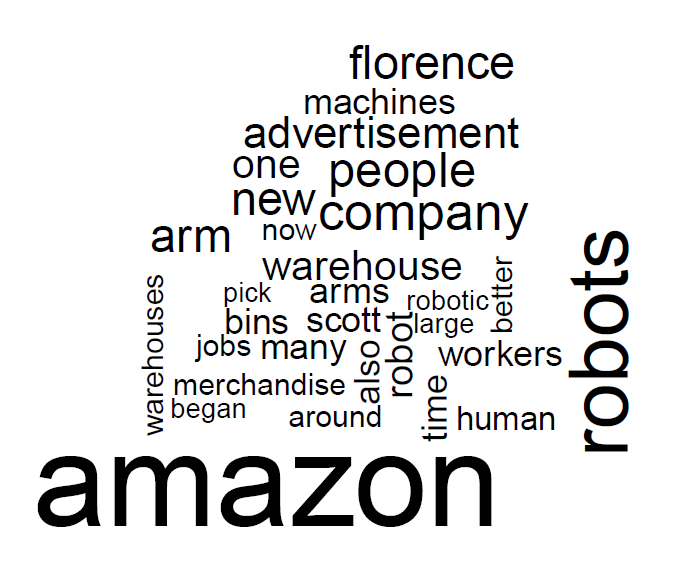
\includegraphics[width = 0.4\textwidth]{figure_man/wordcloud02.png}
\end{center}


%<<echo = F, fig.align='center'>>=
%df = wordmatrix[order(- wordmatrix[, 2]), ]
%df = as.data.frame(df[1:30, ])

%wordcloud(df$word,df$topic2)
%@

\end{vbframe}

\begin{vbframe}{Topic Extraction: Coefficient matrix $\mathbf{H}$}

\footnotesize
\vspace{0.3cm}
\begin{verbatim}
H

##         topic 1   topic 2
## doc1    4.5e+02   1.8e-09
## doc2    2.9e+02   5.8e+01
## doc3    1.6e-09   4.9e+02
\end{verbatim}

%<<echo = F>>=
%H = t(coef(res))
%colnames(H) = c("topic 1", "topic 2")
%@

%<<>>=
%H
%@

\normalsize
The coefficient matrix shows: The first article clearly refers to the first extracted topic, article 3 clearly to the last.
Article 2 addresses both topics.

\vfill

\begin{footnotesize}
Implementation in R: \url{https://rpubs.com/JanpuHou/300168}
\end{footnotesize}

\end{vbframe}

\endlecture
\end{document}







